\chapter{Concentration Inequalities}
\setcounter{section}{-1}   % sections start at 1.0 (see main.tex comment)
\label{ch:conc}

\begin{objectives}
\item Recognize when a component needs a \emph{whp} contract, and formalize the bad event.
\item Prove the ladder Markov $\to$ Chebyshev $\to$ Chernoff/Hoeffding, and match each rung
  to the dependence structure.
\item Tune per-event failure to $\delta/(\text{events})$; union-bound over all copies.
\item Dissect a paper's argument: random object, independence, rung, $\delta$ budget.
\end{objectives}

Concentration inequalities bound the probability that a random quantity strays far from
its expectation. For a systems paper they upgrade a randomized component that is correct
\emph{in expectation} --- a sampler, sketch, random walk, or noise mechanism --- into one
correct \emph{with high probability (whp)}: a quantified contract such as
``$(1\pm\varepsilon)$-accurate with probability $1-1/\operatorname{poly}(n)$'' or
``running time $O(T)$ with probability $1-1/N$.'' The recipe is constant: name the bad
event, bound it by a tail inequality, union-bound over all copies of the component. In the
SIGMOD'26 corpus this is among the most-used theoretical tools (38 tagged papers),
directly supplying the probabilistic-guarantee property in 25 of them.

This chapter presents the basic ladder and the standard exemplars first;
Section~\ref{sec:conc-advanced} adds the advanced rungs (martingales, two harder
exemplars) as extension reading.

\section{The tool: concentration inequalities}

The problem class is uniform across applications: we can compute (or bound) the
expectation of some random quantity $X$ --- the number of sampled points falling in a
region, the error of a private estimate, the load of a hash bucket --- but an algorithm
must succeed on the \emph{actual} draw, not the average. What concentration delivers is a
bound of the form
\[
\Pr\bigl[\,|X - \mathbb{E}X| \ge t\,\bigr] \;\le\; \text{some decreasing function of } t,
\]
plus the craft of making that function decrease fast enough. How fast is ``fast enough''
is the organizing question of this chapter: a bound of $\delta$ per bad event survives a
union bound over $1/\delta$ events, so a component replicated $\operatorname{poly}(n)$
times needs per-event failure $1/\operatorname{poly}(n)$, which in turn needs tails that
decay \emph{exponentially} in the deviation.

\begin{remarkbox}[Notation]
``whp'' (with high probability) always means probability at least
$1 - 1/\operatorname{poly}(n)$, or $1 - 1/N$ for a system of $N$ components; the
polynomial in the failure probability is set by the union bound over the whole system.
\end{remarkbox}

\subsection{The basic ladder}
\label{sec:conc-ladder}

Every bound in the family is Markov's inequality in disguise
\cite{concentration-ineq-bg5,concentration-ineq-bg6,concentration-ineq-bg7}.

\begin{theorem}[Markov]\label{thm:conc-markov}
Let $X \ge 0$ be a random variable with $\mathbb{E}X < \infty$. Then for every $a > 0$,
\[
\Pr[X \ge a] \;\le\; \frac{\mathbb{E}X}{a}. \eopm
\]
\end{theorem}

\begin{proof}
$\mathbb{E}X \ge \mathbb{E}[X \cdot \mathbf{1}\{X \ge a\}] \ge a\,\Pr[X \ge a]$; divide by $a$.
\end{proof}

One moment, one side, polynomial tail. Applying it to $(X-\mu)^2$ instead of $X$ gives the
two-sided, second-moment rung:

\begin{corollary}[Chebyshev]\label{cor:conc-chebyshev}
Let $\mu = \mathbb{E}X$ and $\operatorname{Var}(X) < \infty$. Then for every $t > 0$,
\[
\Pr[\,|X - \mu| \ge t\,] \;\le\; \frac{\operatorname{Var}(X)}{t^2}. \eopm
\]
\end{corollary}

\begin{proof}
Markov (Theorem~\ref{thm:conc-markov}) applied to the nonnegative variable $(X-\mu)^2$
with $a = t^2$.
\end{proof}

Polynomial tails suffice for constant success probability --- boosted to high probability
by repetition and medians --- but they cannot survive a union bound over
$\operatorname{poly}(n)$ events. Exponential tails come from applying Markov to
$e^{\lambda X}$:

\begin{lemma}[Chernoff method]\label{lem:conc-chernoff-method}
For any random variable $X$, any $a \in \mathbb{R}$ and any $\lambda > 0$,
\[
\Pr[X \ge a] \;=\; \Pr\bigl[e^{\lambda X} \ge e^{\lambda a}\bigr] \;\le\;
e^{-\lambda a}\,\mathbb{E}\bigl[e^{\lambda X}\bigr],
\]
and one optimizes over $\lambda > 0$ (the \emph{moment generating function} controls the
tail). \eop
\end{lemma}

\begin{proof}
Markov (Theorem~\ref{thm:conc-markov}) applied to the nonnegative variable
$e^{\lambda X}$ at level $a' = e^{\lambda a}$; the inequality is monotone in $\lambda$'s
sign, so only $\lambda > 0$ is useful.
\end{proof}

Evaluating the moment generating function of a sum of independent bounded variables
yields the two workhorses of randomized systems. The multiplicative form is the one to
memorize for sampling and sketching
\cite{concentration-ineq-bg1,concentration-ineq-bg5,concentration-ineq-bg7}:

\begin{theorem}[Chernoff, multiplicative form]\label{thm:conc-chernoff-mult}
Let $X_1,\dots,X_m$ be independent random variables with $X_i \in [0,1]$,
$X = \sum_{i=1}^m X_i$, $\mu = \mathbb{E}X$. Then for every $\varepsilon \in (0,1)$,
\[
\Pr[X \ge (1+\varepsilon)\mu] \;\le\; e^{-\varepsilon^2\mu/3},
\qquad
\Pr[X \le (1-\varepsilon)\mu] \;\le\; e^{-\varepsilon^2\mu/2}. \eopm
\]
\end{theorem}

\begin{proof}[Proof idea]
Chernoff method (Lemma~\ref{lem:conc-chernoff-method}) on $X$, then the elementary bound
$(1+\varepsilon)\ln(1+\varepsilon)-\varepsilon \ge \varepsilon^2/3$ (and its lower-tail
twin) on the optimized exponent; the full derivation is in the
Appendix (Section~\ref{sec:conc-appendix}).
\end{proof}

The additive form is interchangeable whenever the summands are bounded but not
naturally counts \cite{concentration-ineq-bg2,concentration-ineq-bg7,concentration-ineq-bg8}:

\begin{theorem}[Hoeffding, additive form]\label{thm:conc-hoeffding}
Let $X_1,\dots,X_m$ be independent with $X_i \in [a_i,b_i]$ a.s.\ and
$X = \sum_i X_i$. Then for every $t > 0$,
\begin{align*}
\Pr[X - \mathbb{E}X \ge t] \;&\le\;
\exp\!\Bigl(-\, \frac{2t^2}{\sum_i (b_i-a_i)^2}\Bigr),\\
\Pr[X - \mathbb{E}X \le -t] \;&\le\;
\exp\!\Bigl(-\, \frac{2t^2}{\sum_i (b_i-a_i)^2}\Bigr). \eopm
\end{align*}
\end{theorem}

\begin{proof}[Proof idea]
Chernoff method plus \emph{Hoeffding's lemma},
$\mathbb{E}[e^{\lambda(X_i - \mathbb{E}X_i)}] \le e^{\lambda^2(b_i-a_i)^2/8}$; optimize
$\lambda$ (proof in Section~\ref{sec:conc-appendix}).
\end{proof}

\begin{widefigure}[t]
\pgfplotsset{compat=1.15}
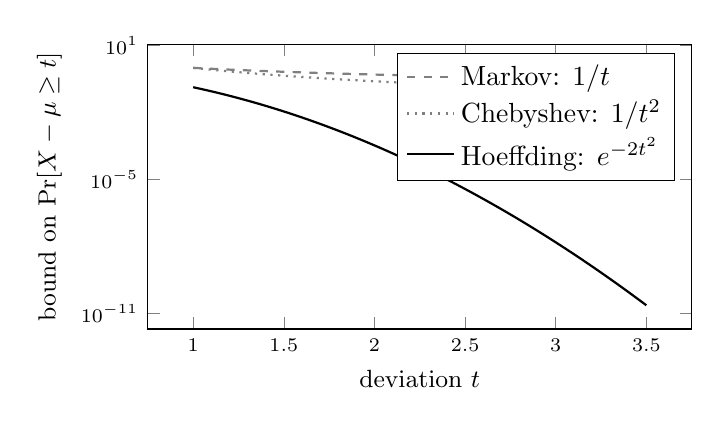
\begin{tikzpicture}
\begin{axis}[
  width=0.7\textwidth, height=5.2cm,
  xlabel={deviation $t$}, ylabel={bound on $\Pr[X-\mu \ge t]$},
  ymode=log, domain=1:3.5, samples=80,
  legend pos=north east, legend cell align=left,
  tick label style={font=\scriptsize}, label style={font=\small}
]
\addplot[gray, thick, dashed]  {1/x};
\addlegendentry{Markov: $1/t$}
\addplot[gray, thick, dotted]  {1/x^2};
\addlegendentry{Chebyshev: $1/t^2$}
\addplot[black, thick]         {exp(-2*x^2)};
\addlegendentry{Hoeffding: $e^{-2t^2}$}
\end{axis}
\end{tikzpicture}
\caption{Tail decay for a unit-scale random quantity: moment bounds fall polynomially,
independence buys the exponential curve --- the gap that makes
$\operatorname{poly}(n)$-way union bounds affordable.}
\label{fig:conc-tails}
\end{widefigure}

\sidenote{The entry fee for both forms is \emph{independence plus bounded summands}. The
tunable currency is the exponent --- $\varepsilon^2\mu$ or $2t^2/\sum_i(b_i-a_i)^2$ ---
which must be pushed past $\log(\text{\#events}/\delta)$ for the failure probability to
amortize. When the summands are unbounded but light-tailed (Gaussian, Laplace,
sub-exponential, sub-gamma), the same Chernoff-method machinery applies with a
moment-generating function that exists near $0$; corpus papers use sub-gamma tails for
approximate counters (Morris-type) and Laplace tails for privacy noise, and we will see
the latter in Section~\ref{sec:conc-ldp}.}

When independence fails but each random choice shifts the running statistic by a bounded
amount, the ladder has two more rungs --- Azuma--Hoeffding and McDiarmid --- built on
martingales; they are stated, with usage guidance, in
Section~\ref{sec:conc-advanced}.

\subsection{How to choose a rung}
\label{sec:conc-choose}

The selection procedure is mechanical once two questions are answered. \emph{First, what
depends on what?} If the random object is a sum of independent bounded indicators ---
samples retained, points in a region, hashed keys --- use multiplicative Chernoff when
the bound should be relative to the expectation $\mu$ (sampling rates, subsampling), and
additive Hoeffding when it should be relative to the range parameters
$b_i - a_i$ (weighted sums, real-valued measurements). \emph{Second, what moments are
available?} If only the mean (or an exponent-optimized mean of a transform) is
computable, Markov is the floor --- and, applied to $e^{\lambda X}$, it is secretly the
ceiling too.

\begin{reachbox}{When to Reach for Concentration}
Reach whenever a randomized component must be certified --- sampling/sketching estimators,
random walks, sampled data structures, hashing, privacy noise --- and the deliverable is a
probability-qualified contract: accuracy $(1\pm\varepsilon)$ whp, or time/space bounds
holding with probability $1-1/N$. Then run the recipe:
\begin{enumerate}
\item Name the random object $X$ and the bad event $\{|X - \mathbb{E}X| \ge t\}$.
\item Check the dependence structure: independent bounded summands $\to$
  Chernoff/Hoeffding; adaptive exposure or capped per-variable influence $\to$ the
  martingale rungs of Section~\ref{sec:conc-advanced}; only moments available $\to$
  Markov/Chebyshev --- constant probability, boostable by repetition with medians (and
  Markov on $e^{\lambda X}$ is the engine of every exponential-tail argument anyway).
\item Tune parameters so each bad event fails with probability at most
  $\delta/(\text{events})$ --- i.e.\ push the exponent past
  $\log(\text{events}/\delta)$; only exponential tails amortize over
  $\operatorname{poly}(n)$ copies, polynomial ones do not.
\item Union-bound over all copies of the component.
\end{enumerate}
\end{reachbox}

\section{Trimmed statistics in a turnstile stream}
\label{sec:conc-trimmed}

The exemplar is a PODS'26 paper on robust streaming statistics \cite{sigmod26-175}\pods.
Frequency moments, $F_p = \sum_i |x_i|^p$, are the workhorses of database analytics:
query optimization, data mining, and network monitoring all rely on them, and the
classical streaming results estimate them over the \emph{whole} frequency vector. Many
analytics tasks, however, want order-restricted quantities instead: statistics built from
only the heaviest (or the central) part of the data, with the extremes treated as
outliers --- the streaming analogue of the trimmed mean from robust statistics. The paper
studies such \emph{trimmed statistics} --- notably the $F_p$ moment of the top-$k$
coordinates, a Ky-Fan-type norm behind impact measures like the $h$-index --- in the
turnstile streaming model, and shows that for every $p \in [0,2]$ they can be estimated
in a single pass using $\operatorname{poly}(\log n/\varepsilon)$ bits of space.

\paragraph{Problem.}
Work in the \emph{strict turnstile} streaming model: an $n$-dimensional frequency vector
$\mathbf{x} \in \mathbb{Z}^n$ starts at zero and receives a long stream of updates of the
form ``add $\Delta$ to coordinate $i$'' (with $\Delta$ of either sign); the algorithm
sees updates one at a time and must answer queries about the final $\mathbf{x}$ using
space far less than $n$. Let $a_1,\dots,a_k$ be the $k$ coordinates of $\mathbf{x}$ of
largest absolute value. The \emph{trimmed statistic} of order $(p,k)$ is
$\sum_{i=1}^k |a_i|^p$ for $0 \le p \le 2$: the $F_p$ mass contributed by the top $k$
coordinates --- the part of the data that survives trimming away the tail. Such
statistics are the streaming analogue of trimmed estimators in robust statistics.

\paragraph{Guarantee.}

\begin{theorem}[Top-$k$ $F_p$ estimation, Theorem~4 of the paper]\label{thm:conc-trimmed}
Let $\mathbf{x} \in \mathbb{Z}^n$, $p \in [0,2]$, $k \ge 0$, $\varepsilon \in (0,1)$.
Suppose $\|\mathbf{x}_{-k}\|_2^2 \ge (\varepsilon/\log n)^c \cdot k$ for a constant $c$,
where $\mathbf{x}_{-k}$ excludes the top-$k$ coordinates. Then there exists a
\emph{linear sketch} using $\operatorname{poly}(\log n/\varepsilon)$ bits of space that
estimates $\sum_{i=1}^k |a_i|^p$ to a $(1\pm\varepsilon)$ factor with high constant
probability. \eop
\end{theorem}

\sidenote{A \emph{linear sketch} stores $A\mathbf{x}$ for a random matrix $A$; it is the
standard route to mergeable, one-pass, deletion-tolerant stream summaries. The condition
on $\|\mathbf{x}_{-k}\|_2^2$ holds automatically once $k \ge \operatorname{polylog} n$,
so the theorem covers the practically interesting regime.}

\paragraph{How concentration is applied.}
The algorithm partitions coordinates by magnitude into \emph{geometric level sets} whose
boundaries are shifted by a random offset $\zeta$ uniform in $[1/2,1]$, then
\emph{dyadically subsamples} each level: each coordinate of level $S_j$ is kept
independently with probability $r = \min\{1,\, C\log n/(\varepsilon^2 s_j)\}$ where
$s_j = |S_j|$ and $C$ is a constant. Survivors are found with a
CountSketch\footnote{CountSketch (Charikar--Chen--Farach-Colton) recovers, from hashed
counters, all coordinates whose value exceeds a $\theta$-fraction of the residual
$\ell_2$ norm (a \emph{heavy hitter} structure); the paper needs only this black box.}
fed with $\Theta(\log n)$ buckets per subsampling rate. The concentration step is the
following lemma; its random objects are the independent retention indicators $X_i$ of
the coordinates of $S_j$, each Bernoulli($r$), so the survivor count has mean $s_j r$.

\begin{lemma}[Level-size estimation, Lemma~4.4 of the paper, notation cleaned]
\label{lem:conc-trimmed-level}
Let $S_j$ be a level set with $s_j = |S_j|$, and subsample each coordinate independently
with probability $r = \min\{1,\, C\log n/(\varepsilon^2 s_j)\}$. If $z$ coordinates of
$S_j$ survive and $\tilde{s}_j = z/r$, then with probability $1 - 1/\operatorname{poly}(n)$,
\[
(1-\varepsilon)\,s_j \;\le\; \tilde{s}_j \;\le\; (1+\varepsilon)\,s_j . \eopm
\]
\end{lemma}

\begin{proof}[Proof sketch]
Write $u_1,\dots,u_{s_j}$ for the coordinates of $S_j$, and let $X_i$ be the indicator
that $u_i$ is sampled, so $\mathbb{E}\sum_i X_i = s_j r$. Multiplicative Chernoff gives
$\Pr[\,|\sum_i X_i - s_jr| \ge \varepsilon s_j r\,] \le
2\exp(-\varepsilon^2 s_j r/3) \le 2\exp(-C\log n/3) \le 1/\operatorname{poly}(n)$;
divide by $r$. (Full proof in Section~\ref{sec:conc-appendix}.)
\end{proof}

The $\delta$ tuning is explicit: $r$ is chosen exactly so that the Chernoff exponent
$\varepsilon^2 s_j r$ equals $C \log n$, i.e.\ per-level failure $1/\operatorname{poly}(n)$;
there are only $O(\log_{1+\varepsilon} m)$ levels (magnitude scales), so a union bound
over levels preserves the polynomial failure probability. A companion lemma (Lemma~4.5 of
the paper) uses the same Chernoff bound on the binomial survivor count to show that fewer
than $O(\log n/\varepsilon^2)$ coordinates survive per level whp --- which is what makes
the heavy-hitter structure, and hence the space bound,
$\operatorname{poly}(\log n/\varepsilon)$.

\paragraph{What it buys.}
The system gets a one-pass, sublinear-space summary of trimmed statistics --- robust
aggregate mass that ignores the tail --- with a certificate strong enough to union-bound
into larger algorithms; the randomness of the offset $\zeta$ (rather than an adversarial
grid) is what makes the level-set decomposition itself immune to worst-case input
placement.

\section{Maximum range sum by randomized grid shifting}
\label{sec:conc-maxrs}

The exemplar is a SIGMOD'26 paper on spatial query processing \cite{sigmod26-259}. The
\emph{maximum range sum} (MaxRS) problem sits behind every ``find the best location''
query: given weighted points --- customers, incidents, sensors --- and a fixed-size
geometric region $Q$, place $Q$ anywhere in space so that it captures as much total
weight as possible; that placement is where to site a store, a base station, or an
emergency facility. The problem is well studied by both the database and the
computational-geometry communities, and the paper revisits it in three practically
motivated variations: \emph{dynamic} MaxRS, where points are inserted and deleted and a
good placement must be maintained under updates; \emph{batched} MaxRS, where many query
regions must be answered at once; and \emph{colored} variants that group the points into
classes. Its headline results are a randomized $(\tfrac12-\varepsilon)$-approximation
for dynamic MaxRS with polylogarithmic update time --- the first algorithm of this kind
--- together with conditional lower bounds showing that the batched problem cannot be
solved substantially faster than the trivial approach.

\paragraph{Problem.}
In the \emph{maximum range sum} (MaxRS) problem, the input is a set $P$ of $n$ points in
$\mathbb{R}^d$, each carrying a weight, and a query shape $Q$ --- here a $d$-ball of
given radius. The goal is to place $Q$ (translate it anywhere) so as to maximize the
total weight of the points of $P$ covered.

Exact MaxRS is expensive: for $Q$ a $2$-ball the colored version carries a conditional
$\Omega(n^2)$ lower bound, and assuming that $(\min,+)$-convolution on length-$n$
sequences requires $\Omega(n^2)$ time, the batched variant on $n$ points and $m$ query
radii requires $\Omega(mn)$ time --- almost matching the trivial $O(mn\log n)$ upper
bound.

\sidenote{\emph{Conditional lower bound}: a reduction from $(\min,+)$-convolution ---
widely conjectured to need quadratic time --- transfers that hardness to MaxRS. This is
the paper's evidence that \emph{approximation} is necessary, and approximation is exactly
where concentration enters.}

\paragraph{Guarantee.}

\begin{theorem}[Static MaxRS, one representative case of the paper]\label{thm:conc-maxrs}
For static MaxRS with $Q$ a $d$-ball and any $0 < \varepsilon < 1/2$, there is a
randomized $(\tfrac12-\varepsilon)$-approximation algorithm running in time
$O(\varepsilon^{-2d-2} n \log n)$; the approximation factor holds with high probability,
i.e.\ $1 - n^{-\Omega(1)}$. The dynamic version achieves the same factor with amortized
update time $O(\varepsilon^{-2d-2}\log n)$. \eop
\end{theorem}

\paragraph{How concentration is applied.}
The algorithm randomly shifts a grid over the point set and, per cell, takes a random
sample of the cell's points; the candidate balls it examines are drawn from a finite set
of $k \le n$ possibilities determined by the shift. Two facts combine. First, a
\emph{geometric covering lemma}: if $C$ is a $d$-ball of radius $\rho$ and $B$ a unit
$d$-ball whose center lies at distance $\rho^2$ from the center of $C$, then the
$(d-1)$-dimensional measure of the cap $B \cap \partial C$ is at least a
$(\tfrac12 - \Theta(\varepsilon))$ fraction of the measure of $\partial C$ --- i.e., a
random point of $C$'s boundary lands in any fixed candidate ball with probability at
least $\tfrac12 - \Theta(\varepsilon)$. Second, the concentration step:

\begin{lemma}[Sampling concentration, Lemma of the paper, notation cleaned]
\label{lem:conc-maxrs-sample}
Let $S = \{p_1,\dots,p_t\}$ be such that each point of $S$ lies inside the candidate ball
$B$ independently with probability at least $\tfrac12 - \Theta(\varepsilon)$, and let
$Y_B = \sum_{i=1}^t \mathbf{1}\{p_i \in B\}$. Then with high probability,
simultaneously for all $k \le n$ candidate balls,
\[
Y_B \;\ge\; (1-\varepsilon)\Bigl(\tfrac12 - \Theta(\varepsilon)\Bigr)\,t . \eopm
\]
\end{lemma}

\begin{proof}[Proof sketch]
The $X_i = \mathbf{1}\{p_i \in B\}$ are independent indicators with
$\mathbb{E}[Y_B] \ge (\tfrac12 - \Theta(\varepsilon))t$; multiplicative Chernoff gives
$\Pr[Y_B < (1-\varepsilon)\mathbb{E}Y_B] \le e^{-\varepsilon^2 t/2}$, and a union bound
over the $k \le n$ balls keeps this whp provided
$t = \Theta(\varepsilon^{-2}\log n)$. (Full proof in
Section~\ref{sec:conc-appendix}.)
\end{proof}

The random objects are the per-point sampling/shift indicators; the structure is full
independence across points (the random shift acts independently per cell); the rung is
multiplicative Chernoff; and the $\delta$ tuning sets $t = \Theta(\varepsilon^{-2}
\log n)$ so each of the $n$ candidate balls fails with probability $n^{-\Omega(1)}$ ---
the same ``push the exponent past $\log(\text{events})$'' accounting as in
Section~\ref{sec:conc-trimmed}, with the exponent coming from sample size rather than
subsample rate.

\paragraph{What it buys.}
The spatial engine answers best-placement queries in near-linear time with a certified
$(1/2-\varepsilon)$ fraction of the optimum whp --- and supports updates in polylog
amortized time --- where exact computation faces (conditional) quadratic barriers. The
same Chernoff-plus-union-bound skeleton, re-instantiated with trapezoidal maps, gives the
paper's $(1-\varepsilon)$-approximation for the colored variant.

\section{User-level private query processing with sampled tuples}
\label{sec:conc-s4s}

The exemplar is a SIGMOD'26 paper on private query processing \cite{sigmod26-079}.
Answering select--join--aggregate (SJA) queries under differential privacy is a basic
building block of privacy-preserving analytics: the system must return an accurate
aggregate while guaranteeing that no adversary can confidently infer whether any one
\emph{user's} data was present or absent. The state of the art achieves strong,
instance-optimal accuracy at this \emph{user level}, but pays for it by solving
expensive optimization programs over the whole database --- prohibitive at scale.
Sampling is the classic escape hatch, buying a tunable trade-off between accuracy and
computational cost, yet combining it with private processing is subtle: it is unclear
\emph{what} to sample for the best accuracy under a given compute budget, and the
existing mathematical tool chains were not designed with sampling in mind. The paper
builds a scalable user-level-DP SJA engine that privately truncates each heavy user's
contribution and Poisson-samples tuples to accelerate the truncation search, with an
error analysis that cleanly separates sampling error from privacy noise.

\paragraph{Problem.}
Consider a select--project--join--aggregate workload over a relational instance whose
rows belong to \emph{users}, each user contributing many tuples. The privacy contract is
differential privacy at the granularity of users:

\begin{definition}[$\varepsilon$-differential privacy, user level]\label{def:conc-dp}
A randomized mechanism $M$ satisfies $\varepsilon$-\emph{differential privacy} if for all
\emph{neighboring} inputs $D,D'$ and all measurable sets $S$,
\[
\Pr[M(D) \in S] \;\le\; e^{\varepsilon}\,\Pr[M(D') \in S].
\]
For \emph{user-level} DP, ``neighboring'' means \emph{all} tuples of one user added or
removed --- much stricter than tuple-level DP.
\end{definition}

Unbounded per-user contributions then blow up sensitivity, so the system
\cite{sigmod26-079} truncates each user's contribution to a threshold $\tau$ chosen
privately by a search (sparse vector technique), and accelerates the search by
Poisson-sampling tuples at rate $q$ before privatizing.

\sidenote{Poisson sampling also \emph{amplifies} privacy: a mechanism that is
$\varepsilon$-DP on the sample is $(\varepsilon')$-DP on the full data with
$\varepsilon' = \ln(1 + q(e^{\varepsilon}-1)) < \varepsilon$; the paper's
Sample-and-Explore comparison baselines use this. The proof is a binomial tail
computation --- again concentration.}

\paragraph{Guarantee.}

\begin{theorem}[Error of the sampled truncation, Algorithm~2 of the paper, compressed]
\label{thm:conc-s4s}
The mechanism satisfies $(\varepsilon,0)$-DP. Let $n$ be the number of records, $m$ the
number of users, and $q$ the sample rate. Write $\tau^*(T) = \max_u \sum_{t \in T}
\mathbf{1}[u \prec t]$ for the true maximum per-user contribution, and
$\varepsilon_i^* \ge \varepsilon/L$ for the noise-calibration budget over the $L$
search iterations. With probability $1-\beta$, the released answer $\hat{f}(T)$ obeys
\[
\bigl|\hat{f}(T) - f(T)\bigr| \;=\;
\widetilde{O}\Bigl(\sqrt{\textstyle\frac{n}{q}} + \frac1q +
\frac{1}{\varepsilon_i^*}\Bigl(\tau^*(T) + \sqrt{\textstyle\frac{\tau^*(T)}{q}}\Bigr)\Bigr),
\]
where $\widetilde{O}(\cdot)$ hides constants and polylogarithmic factors in $m$ and
$1/\beta$. \eop
\end{theorem}

\paragraph{How concentration is applied.}
The random objects are the independent sampling indicators
$\mathbf{1}\{t \text{ sampled}\} \sim \mathrm{Bernoulli}(q)$ over the $n$ tuples. The
sampled statistic $f(S) = \sum_{t \in T} w_t \mathbf{1}[t \text{ sampled}]$ satisfies
$\mathbb{E}[f(S)] = q\,f(T)$ and
$\operatorname{Var}[f(S)] = q(1-q)\sum_t w_t^2 \le qn$: a sum of independent bounded
variables with an explicit variance proxy --- the territory of the Bernstein/Chernoff
rung, whose bound gives $|f(S) - qf(T)| \lesssim \sqrt{qn \log(3L/\beta)}$ with
probability $1 - \beta/(3L)$; dividing by $q$ yields the $\sqrt{n/q}$ term. The
$\delta$-budgeting is again structural: the truncation-threshold search runs $L$
iterations, each is allocated failure probability $\beta/(3L)$, and a union bound over
iterations upgrades the per-iteration bound to the global $1-\beta$ contract --- with the
same per-event log factor $\log(3L/\beta)$ appearing inside the noise scale. The
$\tau^*(T)/\varepsilon_i^*$ terms come from the Laplace-style calibration of the final
release against the (privately learned) per-user cap.

\paragraph{What it buys.}
The query engine can offer user-level --- not merely tuple-level --- privacy at a
modest accuracy price: the sampling error $\sqrt{n/q}$ decouples from the privacy noise,
so tuning $q$ trades compute for accuracy without touching the privacy guarantee, and
the explicit $\tau^*(T)$ dependence quantifies exactly how much heavy user-contributors
cost the answer.

\section{Advanced usage and further reading}
\label{sec:conc-advanced}

Everything so far needs independence. Two extensions belong in every practitioner's
backpack: the martingale rungs that replace independence with bounded per-step
influence, and the light-tailed regime where summands are unbounded but have a moment
generating function. This section states the rungs, sketches two harder exemplars, and
points to the literature.

\subsection{Martingale rungs: Azuma--Hoeffding and McDiarmid}
\label{sec:conc-martingales}

Expose the randomness sequentially and book the shifts as a
\emph{martingale}\footnote{Recall: a martingale difference sequence $(Y_i)$ with respect
to a filtration $(\mathcal{F}_i)$ has $\mathbb{E}[Y_i \mid \mathcal{F}_{i-1}] = 0$; the
partial sums $M_j = \sum_{i\le j} Y_i$ then satisfy $\mathbb{E}[M_j \mid
\mathcal{F}_{j-1}] = M_{j-1}$.}:

\begin{theorem}[Azuma--Hoeffding]\label{thm:conc-azuma}
Let $(Y_i)_{i=1}^m$ be a martingale difference sequence with $|Y_i| \le c_i$ a.s. Then
for every $t > 0$,
\[
\Pr\Bigl[\textstyle\sum_{i=1}^m Y_i \ge t\Bigr] \;\le\;
\exp\!\Bigl(-\, \frac{t^2}{2\sum_{i=1}^m c_i^2}\Bigr). \eopm
\]
\end{theorem}

\begin{proof}[Proof idea]
Chernoff method on $\sum_i Y_i$, Hoeffding's lemma applied to each $Y_i$
\emph{conditionally on the past} (boundedness is all that is needed; independence is
replaced by iterated conditioning), then optimize $\lambda$
(Section~\ref{sec:conc-appendix}).
\end{proof}

The function-of-independent-variables form is the rung most used for adaptive
algorithms and data structures, where the analyzed quantity is not a sum but a function
whose per-variable influence is capped
\cite{concentration-ineq-bg4,concentration-ineq-bg5,concentration-ineq-bg6}:

\begin{theorem}[McDiarmid, bounded differences]\label{thm:conc-mcdiarmid}
Let $X_1,\dots,X_m$ be independent random variables and
$f\colon \prod_i \mathcal{X}_i \to \mathbb{R}$ a measurable function satisfying the
bounded differences condition: for each $i$ there is $c_i \ge 0$ with
\[
\bigl|f(x_1,\dots,x_i,\dots,x_m) - f(x_1,\dots,x_i',\dots,x_m)\bigr| \;\le\; c_i
\]
for all inputs and all $x_i'$. Then for every $t > 0$,
\[
\Pr\bigl[f(X_1,\dots,X_m) - \mathbb{E}f \ge t\bigr] \;\le\;
\exp\!\Bigl(-\, \frac{2t^2}{\sum_{i=1}^m c_i^2}\Bigr). \eopm
\]
\end{theorem}

\begin{proof}[Proof idea]
Apply Azuma--Hoeffding (Theorem~\ref{thm:conc-azuma}) to the \emph{Doob martingale}
$Y_i = \mathbb{E}[f \mid X_1,\dots,X_i] - \mathbb{E}[f \mid X_1,\dots,X_{i-1}]$, whose
increments are bounded by $c_i$ exactly because changing $X_i$ moves $f$ by at most
$c_i$ (Section~\ref{sec:conc-appendix}).
\end{proof}

\emph{When these rungs earn their keep.} If the algorithm is \emph{adaptive} --- later
random choices conditioned on earlier estimates, sampling without replacement, stopping
times --- the summands are dependent but each step's effect is bounded, and
Azuma--Hoeffding applies. If the quantity is a \emph{function} of many independent
inputs (a data structure's quality, a clustering cost, a query plan's runtime) with
per-input influence at most $c_i$, McDiarmid converts that directly. Hashing with
limited independence is the classic gap: the indicators are not fully independent, but
exposure by hash key gives bounded increments.

\subsection{Two advanced exemplars, sketched}
\label{sec:conc-ldp}

Both exemplars of this section are privacy papers that push past the
sum-of-independent-bounded-summands regime; each is sketched in one paragraph, and the
round-by-round argument of the first is transcribed in the
Appendix (Section~\ref{sec:conc-appendix}).

\paragraph{Private graph pattern counting under LDP \cite{sigmod26-012}.}
Counting subgraph patterns --- triangles, paths, stars --- is a cornerstone of network
analysis (community detection, fraud detection), and releasing such counts leaks
information about individual edges. Under \emph{local} differential privacy there is no
trusted curator: each node of the graph randomizes its own messages before anything is
aggregated, and existing LDP mechanisms were ad hoc, handling only specific patterns
such as triangles and stars. The paper gives the first general mechanism for counting
arbitrary \emph{acyclic} patterns under LDP. It runs $k$ rounds of message passing,
adding fresh Laplace noise --- \emph{sub-exponential} tails, so the Chernoff method
still applies --- at every node in every round. The $\delta$-accounting is the recipe of
Section~\ref{sec:conc-choose} in its purest form: failure budget $\beta'/N$ per node
per round, union bound over the $kN$ node-rounds, then an \emph{induction on rounds}
that grows the noise scale geometrically but controllably. The resulting estimate is
unbiased with error $\widetilde{O}(\sqrt{N\,d(G)^{k-1}})$ --- the square root of the
maximal possible count. For simple paths, the tail is only polynomial in $1/\beta$
(a variance/Markov argument), illustrating the price of dropping exponential tails.

\label{sec:conc-product}
\paragraph{Product noise as a concentration bound \cite{sigmod26-196}.}
Adding calibrated noise to a released statistic is the most fundamental route to
differential privacy: the system outputs $f(x) + \mathbf{n}$, and the guarantee rests
on the tail of the \emph{privacy-loss random variable} $L_M = \ln\frac{dP}{dQ}$ ---
$(\varepsilon,\delta)$-DP holds exactly when $\Pr[L_M \ge \varepsilon] \le \delta$,
a tail bound in disguise. For Gaussian noise $L_M$ is itself a univariate Gaussian,
and this is where standard analyses stop. The paper instead exploits the spherical
symmetry of typical noise distributions to generate $\mathbf{n}$ from a
\emph{product} of two independent components --- a radius controlling the noise
magnitude and a direction controlling its angle relative to the sensitivity vector
--- which re-expresses $L_M$ as a product measure and lets the tail be optimized
directly. The paper never writes the word ``Chernoff,'' but its argument --- factorize
$L_M$ into independent terms, bound $\mathbb{E}[U^q]$ for a transform $U$, and
\emph{minimize the resulting $\delta$ over the exponent $q$} --- is exactly the
Chernoff method (Lemma~\ref{lem:conc-chernoff-method}) on a likelihood ratio. The
payoff: expected noise smaller by a $\Theta(\log(1/\delta))$ factor than the Gaussian
mechanism at equal privacy.

\subsection{Further reading}

\begin{itemize}
\item Boucheron, Lugosi, and Massart \cite{concentration-ineq-bg5} --- the comprehensive
non-asymptotic treatment; the martingale and supremum versions live here.
\item Dubhashi and Panconesi \cite{concentration-ineq-bg6} --- the
randomized-algorithms viewpoint, with the exposure/Doob-martingale technique foregrounded.
\item Mitzenmacher and Upfal \cite{concentration-ineq-bg8} --- textbook treatment with
CS applications and all the Chernoff variants used in systems papers.
\item The originals: Chernoff (1952) \cite{concentration-ineq-bg1}, Hoeffding (1963)
\cite{concentration-ineq-bg2}, Azuma (1967) \cite{concentration-ineq-bg3}, and
McDiarmid's bounded-differences survey \cite{concentration-ineq-bg4}.
\item For a two-page refresher with proofs of the additive forms, the Stanford CS229
notes \cite{concentration-ineq-bg7}.
\end{itemize}

\begin{recap}
\item \textbf{What the tool is.} Concentration inequalities convert expectations into
  with-high-probability contracts: $\Pr[|X - \mathbb{E}X| \ge t]$ bounded by a tail
  function, tuned so that per-event failure $\delta/(\text{events})$ survives a union
  bound over all copies of the randomized component.
\item \textbf{Which rung when.} Independent bounded indicators/sums: multiplicative
  Chernoff (relative error) or additive Hoeffding (range-based). Adaptive or dependent
  exposure with bounded per-step effect: Azuma--Hoeffding. Function of many independent
  inputs with capped per-input influence: McDiarmid. Only moments available: Markov and
  Chebyshev --- constant-probability results, boostable by medians. Light-tailed
  unbounded noise (Laplace, Gaussian, sub-gamma): the Chernoff method still applies via
  the moment generating function.
\item \textbf{Why exponential tails.} Only $e^{-\Omega(\text{exponent})}$ tails make
  $\operatorname{poly}(n)$-way union bounds affordable; polynomial tails ($1/t$,
  $1/t^2$) cannot amortize --- visible in the corpus as the gap between
  $\widetilde{O}(\cdot)$ guarantees (Laplace/Chernoff paths) and $1/\beta$-type errors
  (variance-only paths).
\item \textbf{What the corpus showed.} Trimmed-statistic sketching
  (Section~\ref{sec:conc-trimmed}): Chernoff on subsampling survivors, union over
  $O(\log_{1+\varepsilon} m)$ levels. Spatial MaxRS (Section~\ref{sec:conc-maxrs}):
  Chernoff on sampled point-in-ball indicators, union over $\le n$ candidate balls.
  User-level private queries (Section~\ref{sec:conc-s4s}): Bernstein/Chernoff on
  Bernoulli-sampled sums with $\beta/(3L)$ budgets over search iterations.
\item \textbf{Advanced usage.} The martingale rungs
  (Section~\ref{sec:conc-martingales}) replace independence with bounded per-step
  influence; the privacy exemplars of Section~\ref{sec:conc-ldp} run the Chernoff
  method on Laplace noise and on a likelihood ratio. Long proofs of everything
  deferred live in the Appendix (Section~\ref{sec:conc-appendix}).
\end{recap}

\section{Appendix}
\label{sec:conc-appendix}

Proofs omitted from the main text are collected here.

\subsubsection*{Proof of Theorem~\ref{thm:conc-chernoff-mult} (Chernoff, multiplicative form)}
{\itshape Statement (recalled).} Let $X_1,\dots,X_m$ be independent with
$X_i \in [0,1]$, $X = \sum_i X_i$, $\mu = \mathbb{E}X$. Then
$\Pr[X \ge (1+\varepsilon)\mu] \le e^{-\varepsilon^2\mu/3}$ and
$\Pr[X \le (1-\varepsilon)\mu] \le e^{-\varepsilon^2\mu/2}$.\eop

\begin{proof}
By the Chernoff method (Lemma~\ref{lem:conc-chernoff-method}), for $\lambda > 0$,
$\Pr[X \ge (1+\varepsilon)\mu] \le e^{-\lambda(1+\varepsilon)\mu}
\prod_i \mathbb{E}[e^{\lambda X_i}]$. For $X_i \in [0,1]$ independence gives
$\mathbb{E}[e^{\lambda X_i}] = 1 + p_i(e^{\lambda}-1) \le
\exp(p_i(e^{\lambda}-1))$, so the product is at most $e^{\mu(e^\lambda - 1)}$ and,
choosing $\lambda = \ln(1+\varepsilon)$,
\[
\Pr[X \ge (1+\varepsilon)\mu] \;\le\;
\Bigl(\frac{e^{\varepsilon}}{(1+\varepsilon)^{1+\varepsilon}}\Bigr)^{\mu}
\;\le\; e^{-\varepsilon^2\mu/3},
\]
using $(1+\varepsilon)\ln(1+\varepsilon) - \varepsilon \ge \varepsilon^2/3$ for
$\varepsilon \in (0,1)$. The lower tail is symmetric, with exponent
$\varepsilon^2/2$.
\end{proof}

\subsubsection*{Proof of Theorem~\ref{thm:conc-hoeffding} (Hoeffding, additive form)}
{\itshape Statement (recalled).} Let $X_1,\dots,X_m$ be independent with
$X_i \in [a_i,b_i]$ a.s.\ and $X = \sum_i X_i$. Then for every $t > 0$,
$\Pr[X - \mathbb{E}X \ge t] \le \exp(-2t^2/\sum_i (b_i-a_i)^2)$, and the same for the
lower tail.\eop

\begin{proof}
\emph{Hoeffding's lemma}: if $Y \in [a,b]$ a.s.\ and $\mathbb{E}Y = 0$, then
$\mathbb{E}[e^{\lambda Y}] \le e^{\lambda^2(b-a)^2/8}$. (Proof: $e^{\lambda y}$ is
convex, so $e^{\lambda Y} \le \frac{b-Y}{b-a}e^{\lambda a} + \frac{Y-a}{b-a}e^{\lambda
b}$ pointwise; take expectations and minimize over a shifted $\lambda$.) Applying the
lemma to each centered summand and multiplying by independence,
$\mathbb{E}[e^{\lambda(X - \mathbb{E}X)}] \le e^{\lambda^2 \sum_i (b_i-a_i)^2/8}$; the
Chernoff method then gives
$\Pr[X - \mathbb{E}X \ge t] \le e^{-\lambda t + \lambda^2\sum(b_i-a_i)^2/8}$, and
optimizing at $\lambda = 4t/\sum(b_i-a_i)^2$ yields the stated
$e^{-2t^2/\sum(b_i-a_i)^2}$.
\end{proof}

\subsubsection*{Proof of Theorems~\ref{thm:conc-azuma} and~\ref{thm:conc-mcdiarmid} (martingale rungs)}
{\itshape Statement (recalled).} (i) If $(Y_i)_{i=1}^m$ is a martingale difference
sequence with $|Y_i| \le c_i$ a.s., then $\Pr[\sum_i Y_i \ge t] \le
\exp(-t^2/2\sum_i c_i^2)$. (ii) If $f$ has bounded differences $(c_i)$ over independent
$X_1,\dots,X_m$, then $\Pr[f - \mathbb{E}f \ge t] \le
\exp(-2t^2/\sum_i c_i^2)$.\eop

\begin{proof}
Let $M_j = \sum_{i \le j} Y_i$ with $\mathbb{E}[Y_i \mid \mathcal{F}_{i-1}] = 0$ and
$|Y_i| \le c_i$. Iterated conditioning gives
$\mathbb{E}[e^{\lambda M_m}] = \mathbb{E}[e^{\lambda M_{m-1}}
\mathbb{E}[e^{\lambda Y_m} \mid \mathcal{F}_{m-1}]]$, and \emph{conditionally on
$\mathcal{F}_{m-1}$} the variable $Y_m$ is centered and bounded in an interval of length
$2c_m$, so Hoeffding's lemma applies with $(b-a) = 2c_m$. Unrolling,
$\mathbb{E}[e^{\lambda M_m}] \le e^{\lambda^2\sum c_i^2/2}$, and optimizing $\lambda$
gives the stated tail. For McDiarmid, set $Y_i = \mathbb{E}[f \mid X_1,\dots,X_i] -
\mathbb{E}[f \mid X_1,\dots,X_{i-1}]$: this is a martingale difference sequence with
$|Y_i| \le c_i$ precisely because resampling only $X_i$ moves $f$ by at most $c_i$
(take conditional expectations over the two values of $X_i$), and
$\sum_i Y_i = f - \mathbb{E}f$. Azuma--Hoeffding applied to $(Y_i)$ is McDiarmid's
inequality.
\end{proof}

\subsubsection*{Proof of Lemma~\ref{lem:conc-trimmed-level} (level-size estimation,
Section~\ref{sec:conc-trimmed})}
{\itshape Statement (recalled).} Subsample each coordinate of a level set $S_j$,
$|S_j| = s_j$, independently with probability $r = \min\{1, C\log n/(\varepsilon^2
s_j)\}$. If $z$ coordinates survive, then $\tilde{s}_j = z/r$ satisfies
$(1-\varepsilon)s_j \le \tilde{s}_j \le (1+\varepsilon)s_j$ with probability
$1 - 1/\operatorname{poly}(n)$.\eop

\begin{proof}
Denote the coordinates of $S_j$ by $u_i$, $i \in [s_j]$, and let $X_i$ be the indicator
that $u_i$ is sampled into substream $P$, so the $X_i$ are independent with
$\mathbb{E}[X_i] = r$ and $\mathbb{E}\sum_i X_i = s_j r$. Multiplicative Chernoff
(Theorem~\ref{thm:conc-chernoff-mult}) gives
\begin{align*}
\Pr\Bigl[\Bigl|\textstyle\sum_i X_i - s_j r\Bigr| \ge \varepsilon s_j r\Bigr]
\;&\le\; 2\exp(-\varepsilon^2 s_j r/3)
\;\le\; 2\exp(-C\log n/3)\\
\;&\le\; 1/\operatorname{poly}(n),
\end{align*}
where the second inequality uses $s_j r = C\log n/\varepsilon^2$ (when the minimum in
the definition of $r$ is attained at this branch; otherwise $r = 1$ and there is nothing
to estimate). Dividing by $r$ converts the event into
$(1-\varepsilon)s_j \le \tilde{s}_j \le (1+\varepsilon)s_j$.
\end{proof}

\subsubsection*{Proof of Lemma~\ref{lem:conc-maxrs-sample} (sampling concentration,
Section~\ref{sec:conc-maxrs})}
{\itshape Statement (recalled).} If each point of $S = \{p_1,\dots,p_t\}$ lies in the
candidate ball $B$ independently with probability at least
$\tfrac12 - \Theta(\varepsilon)$, then simultaneously for all $k \le n$ candidate
balls, $Y_B = \sum_i \mathbf{1}\{p_i \in B\} \ge
(1-\varepsilon)(\tfrac12 - \Theta(\varepsilon))t$ whp.\eop

\begin{proof}
Fix a candidate ball $B$ and let $X_i = \mathbf{1}\{p_i \in B\}$; the $X_i$ are
independent, and by the covering property $\mathbb{E}[Y_B] = \sum_i \mathbb{E}X_i \ge
(\tfrac12 - \Theta(\varepsilon))t$. Multiplicative Chernoff gives
\[
\Pr\bigl[Y_B < (1-\varepsilon)\mathbb{E}Y_B\bigr] \;\le\;
e^{-\varepsilon^2 \mathbb{E}Y_B/2} \;\le\; e^{-\Theta(\varepsilon^2 t)}.
\]
With $t = \Theta(\varepsilon^{-2}\log n)$ this is $n^{-\Omega(1)}$ per ball, and a union
bound over the $k \le n$ candidate balls gives the simultaneous statement
$Y_B \ge (1-\varepsilon)(\tfrac12-\Theta(\varepsilon))t$ for all of them, with high
probability.
\end{proof}

\subsubsection*{Round-by-round noise control (Section~\ref{sec:conc-ldp})}
{\itshape Statement (recalled).} The $k$-round walk mechanism of \cite{sigmod26-012} is
unbiased for the walk count $W_k$ and, with probability $1-\beta$, errs by at most
$k\gamma\sqrt{N}\,(d(G)+\gamma)^{k-1}$, where
$\gamma = 2k\sqrt{8\log(2kN/\beta)}/\varepsilon$.\eop

\begin{proof}
Write $X_i^{(\ell)}$ for node $i$'s round-$\ell$ value. The mechanism gives, for each
node $i$ and round $\ell \in \{1,\dots,k\}$,
\[
X_i^{(\ell)} \;=\; \sum_{j \in N(i)} X_j^{(\ell-1)} \;+\;
\mathrm{Lap}\bigl(2k\|X^{(\ell-1)}\|_\infty/\varepsilon\bigr),
\]
so $\sum_{j\in N(i)} X_j^{(\ell-1)} \le d(G)\,\|X^{(\ell-1)}\|_\infty$ always. Allocate
failure $\beta'/N$ per node per round: the Laplace tail
$\Pr[\mathrm{Lap}(b) > u] \le \tfrac12 e^{-u/b}$ gives, with probability
$1-\beta'/N$ per node-round,
$2k\,\mathrm{Lap}(\|X^{(\ell-1)}\|_\infty/\varepsilon) \le
\gamma \|X^{(\ell-1)}\|_\infty$ for the stated $\gamma$ (with
$\beta' \approx \beta/k$). Union-bounding over the $\le kN$ node-rounds, all these
events hold simultaneously with probability $\ge 1-(k-1)\beta'$, and on that event an
induction gives
\[
\|X^{(\ell)}\|_\infty \;\le\; \bigl(d(G)+\gamma\bigr)\,\|X^{(\ell-1)}\|_\infty
\quad\Longrightarrow\quad
\|X^{(\ell)}\|_\infty \;\le\; \bigl(d(G)+\gamma\bigr)^{\ell}
\]
for all $\ell \le k-1$. The released count aggregates the $N$ per-node values, whose
centered Laplace contributions are independent sub-exponential variables each of scale
at most $O(\gamma(d(G)+\gamma)^{k-1})$; their sum concentrates around zero at scale
$\sqrt{N}\cdot\widetilde{O}(\gamma(d(G)+\gamma)^{k-1})$ by the same Chernoff-method
argument applied to light-tailed variables, which yields the stated
$k\gamma\sqrt{N}(d(G)+\gamma)^{k-1}$ error radius with probability $1-\beta$.
\end{proof}

\bibliographystyle{plainnat}
\bibliography{chapters/concentration-ineq-all}
